\documentclass[titlepage]{scrartcl}
\usepackage{enumitem}
\usepackage[british]{babel}
\usepackage[style=apa, backend=biber]{biblatex}
\DeclareLanguageMapping{british}{british-apa}
\usepackage{url}
\usepackage{float}
\restylefloat{table}
\usepackage{perpage}
\MakePerPage{footnote}
\usepackage{abstract}
\usepackage{graphicx}
% Create hyperlinks in bibliography
\usepackage{hyperref}
\usepackage{amsmath}

\usepackage[T1]{fontenc}
\usepackage[utf8]{inputenc}
\usepackage{blindtext}
\setkomafont{disposition}{\normalfont\bfseries}


\graphicspath{
    {./resources/},
}
\addbibresource{~/PerryPerrySource/LaTeX/ExperimentalMusic_Bibliography.bib}

\newsavebox{\abstractbox}
\renewenvironment{abstract}
  {\begin{lrbox}{0}\begin{minipage}{\textwidth}
   \begin{center}\normalfont\sectfont\abstractname\end{center}\quotation}
  {\endquotation\end{minipage}\end{lrbox}%
   \global\setbox\abstractbox=\box0 }

\usepackage{etoolbox}
\makeatletter
\expandafter\patchcmd\csname\string\maketitle\endcsname
  {\vskip\z@\@plus3fill}
  {\vskip\z@\@plus2fill\box\abstractbox\vskip\z@\@plus1fill}
  {}{}
\makeatother

\DeclareCiteCommand{\citeyearpar}
    {}
    {\mkbibparens{\bibhyperref{\printdate}}}
    {\multicitedelim}
    {}

\begin{document}
    \title{Experimental Music\\Summative Assignment 2\\Essay}
    \subtitle{\LARGE{The role of electronic feedback and amplification in
    experimental music composition.}}
    \author{Sam Perry\\U1265119}
    \date{}

    \begin{abstract} 
        The use of electronic feedback as tools for musical composition has
        featured in many composition, popular for it's volatile and
        indeterminate nature.  Intrinsic to the use of feedback is the use of
        amplification, capable of artificially altering an input's energy, as a
        method for feedback control. This essay aims to provide a definition of
        these tools in their different forms, and to analyse their use in a
        range of prominent compositions. Forms of feedback will be defined,
        followed by a discussion of the musical implications of their use,
        including consideration for aspects such as process, indeterminacy,
        spectral implications and rhythmic implications. This will be related
        to a number of compositions in order to provide an overall
        understanding of their role in experimental music composition.
    \end{abstract}

    \maketitle

    \section{Defining feedback and amplification}
    A simple definition of feedback is the process of routing the output of a
    system back to the input of that system.~\parencite[p.1]{weisert2010ioi}
    This can take many form in the context of music, whether it is the acoustic
    feedback created by aiming a microphone to it's amplifier, or the digital
    feedback present in an IIR filter, in all cases a loop is created from an
    output point of a system, back to it's input.\\
    The three types of feedback to be considered are:
    \begin{itemize}
        \item{Acoustic Feedback}
        \item{Electronic Feedback}
        \item{Mathmatical Feedback}
    \end{itemize}
    In order to fully understand feedback, electronic amplification will also
    be explored due to it's integral part in feedback system control.
        
    \subsection{Acoustic Feedback}
    Acoustic feedback occurs when a closed loop is created between an audio
    transducer (such as a microphone or guitar pickup) and amplifier,
    causing previously amplified audio to be reamplified continuously at an
    exponential rate as illustrated in Figure~\ref{acoustic_feedback}.\\
    \begin{figure}
        \makebox[\textwidth]{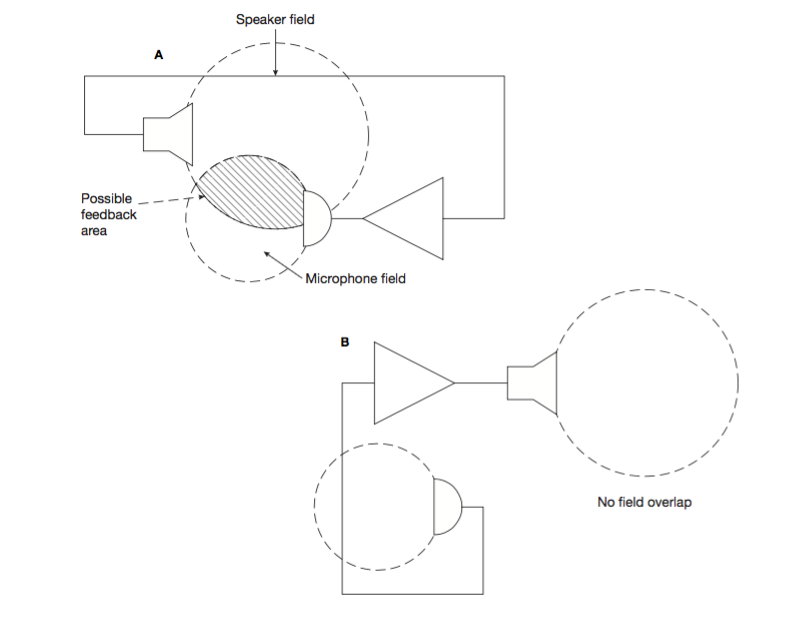
\includegraphics[width=\textwidth]{acoustic_feedback_diagram}}
        \caption[Caption for LOF]{Acoustic Feedback Diagram\protect\footnotemark}
        \label{acoustic_feedback}
    \end{figure}

    \footnotetext{Diagram taken from:~\parencite[p.185]{holmes2012eaem}}

    This is a common problem in the context of live audio, as the exponential
    nature of the feedback causes a distinct "howling" sound that builds
    rapidly and is commonly considered unplesant. As a result, a great deal of
    research has been carried out into methods for attenuating and controlling
    this effect.~\parencite[p.1]{waterschoot2010fyafc} However, the volatile
    and unpredictable nature of acoustic feedback has been used to great effect
    in both popular and avant-garde music.  Pioneering guitarists such as Jimi
    Hendrix have used the loop created through placing an electric guitar
    pickup close to it's amplifier to compliment virtuosic guitar solos in
    pieces such as Foxy Lady~\citeyearpar{} This is taken one step further in
    avante-garde works such as Steve Reich's Pendulum Music, where feedback
    becomes the focus of the piece entirely. This is discussed further in
    section~\ref{pendulum}
    
    \subsection{Electronic Feedback}
    Electronic feedback takes the principal of recursively feeding an output
    back into an input into the analog electronics domain. In this situation,
    the recursive processing is performed purely on electrical signals,
    replacing the initial acoustic input from the microphone found in acoustic
    feedback, with a purely electronic input as part of an electronic circuit.
    The result of this process is then produced in the listening space via
    amplification~\parencite[p.187]{holmes2012eaem}. Composers such as David
    Tudor and Gordon Mumma explore these techniques through their creation and
    use of custom electronic circuits designed to exploit the characteristics
    of this effect.~\parencite[p.186, 390]{holmes2012eaem} A detailed analysis
    of these techniques are presented in section~\ref{ElecFeed}\\

    Although it is outside the scope of this essay, it is worth noting that
    delay feedback forms the basis for electronic IIR filtering, both in the
    analog and digital domain, and by extension is an integral part of almost
    any composition that utilises audio
    filters/equalizers.~\parencite[p.71-72]{zolzer2011dafx} This is an example
    of how the precice control of electronic feedback can lead to a plethora of
    creative musical possibilities.

    \subsection{Amplification}
    Amplification is the process of scaling a signal by a chosen factor.
    Factors $>1.$ result in an increased overall amplitude (a regenerative
    feedback system), whilst factors
    $<1.$ result in an attenuated signal amplitude (a degenerative feedback
    system)~\parencite[p.3-4]{kadis2012sosr}. 
    This artificial modification of amplitude has a number of interesting sonic
    effects in itself, as it allows for the magnification of sounds that may not
    naturally be perceivable and conversely, the reduction of extremely loud
    sounds, to with a comfortable range for hearing. This explored through
    works such as John Cage's Cartridge Music and Stockhausen's Mikrophonie as
    discussed in section~\ref{amp}\\

    It has been stated that feedback (particularly acoustic feedback) is
    difficult to control. This is due to it's recursive nature and the tendancy
    in many situations for output that exceeds unity gain (a state, whereby the
    output amplitude of a feedback system is equal to that of it's input) to be
    fed back into the system. Amplification is therefor a crucial element for
    controlling the results of a feedback system. By attenuating an output
    before feeding it back to a system, it is possible to ensure that outputs
    do not grow at an exponential rate.~\parencite[p.71-72]{zolzer2011dafx}
    \begin{figure}
        \makebox[\textwidth]{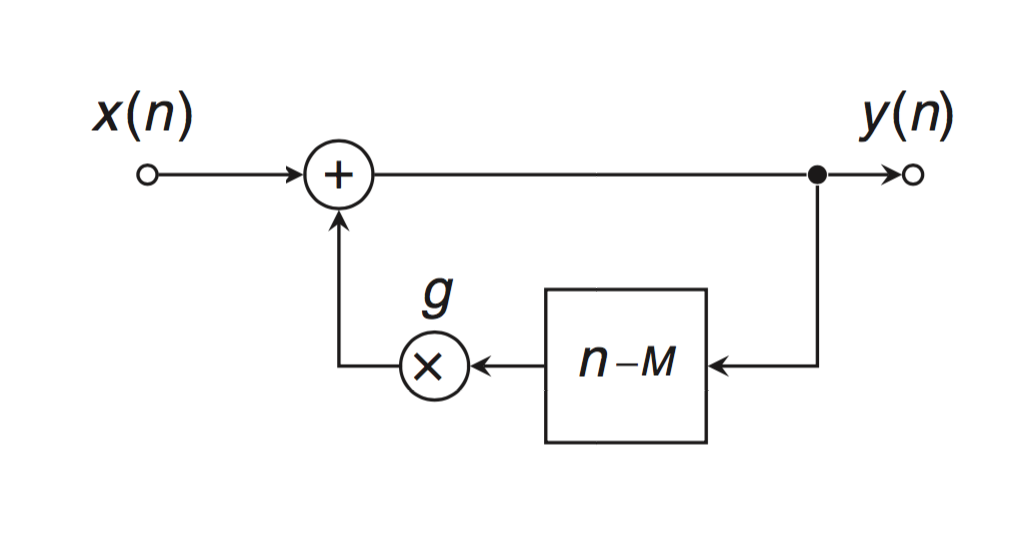
\includegraphics[width=0.75\textwidth]{IIR_flow_diagram}}
        \caption[Caption for LOF]{Basic Feedback Signal Flowchart\protect\footnotemark}
        \label{feed_flowchart}
    \end{figure}

    \footnotetext{Diagram adapted from:~\parencite[p.72]{zolzer2011dafx}}

    \begin{figure}[H]
    This can be demonstrated mathmatically using the following example equation
    for a feedback system as illustrated in figure~\ref{feed_flowchart}:
        \begin{align*}
            & y(n) = x(n) + gy(n-M)\\
            & \text{where:}\\
            & x\text{ is the input signal}\\
            & y\text{ is the output signal}\\
            & n\text{ is the current point in time}\\
            & M\text{ is the signal delay in time}\\
            & g\text{ is the feedback coefficient}\\
        \end{align*}
    \end{figure}
    It is clear that $|g|$ dictates the stability of the signal, as values
    $>1.$ increase exponentially as stated above.~\parencite[p.70-72]{zolzer2011dafx} 

    For example, in the case of acoustic feedback, $g$ is dictated by the
    amount of signal that passes from the amplifier back to the microphone.
    Placing the microphone close will result in a large amount of the amplified
    signal returning to the amplifier, causing further amplification. When the
    system reaches it's limit (which it will do very quickly) the signal
    distorts, causing the typical "howling" effect.

    \subsection{Mathmatical Feedback}
    Mathmatical feedback is not technically a form of electronic feedback and
    so will not be discussed in detail, however it does provide a good example
    of the extent to which the concepts of feedback are used for creative
    purposes in the context of experimental music. 
    Previously discussed feedback methods operate directly on a signal.
    However, mathmatical feedback differs, in that it applies the mathmatical
    principals of feedback to influence musical parameters of the composition.
    This is demonstarted in Tom Johnson's Rational Melody XXI, where Johnson
    specifies each subsequent bar as a retrograde of the previous bar, thus
    causing the composition of each bar to rely on it's
    predecessor.~\parencite[p.72]{weisert2010ioi} This follows the same
    principles as stated in the equation with minor changes:
    \begin{align*}
        & y(n) = x(n) + g \cdot \text{ret}(y(n-M))\\
        & \text{where:}\\
        & \text{ret is a retrograde function}\\
        & g = 1\\
        & n_0 = \text{the initial musical phrase}\\
        & n_{n\neq0} = \text{an empty phrase}
    \end{align*}
    
    \section{Musical Aspects and Implications of Feedback Systems}
    There are a number of interesting musical implications when using feedback
    and amplitude ajustment as a compositional tools. Features, such as it's
    indeterministic nature and rhythmic characteristics, inherent to the nature
    of feedback make it an interesting technique for musical exploration and
    there are many examples of artists exploiting these qualities in
    experimental compositions. Likewise, amplitude modification offers a number
    of compositional possibilities for both the control of feedback and for
    creative effect in of itself. This section outlines some of the key musical
    aspects of feedback and artificial amplification and provides examples of
    notable compositions that demonstrate these principals.

    \subsection{Indeterminacy}\label{indeterminate}
    Indeterminacy is related to the use of chance operations in music
    composition and performance. techniques that involve a degree of
    uncertainty, where external variables or unpredictable factors affect the
    outcome, are defined as indeterminate. Simms describes indeterminacy as
    "Any part of a musical work is indeterminate if it is chosen by chance, or
    if its performance is not precisely
    specified."~\parencite[p.357]{simms1986mtc} It is a topic of interest for
    experimental composers for a number of reasons.

    \subsubsection{Variation in Performance}\label{variance}
    Using indeterministic processes as part of a composition allows for
    variation in the performance of said composition on a case by case basis.
    Through the addition of random factors to a composition, far greater
    degrees of variance are created in the performance of a peice, allowing for
    an infinite number of possible versions as opposed to the comparatively
    limited interpretation of static compositions where all elements are
    controlled directly by the composer.~\parencite[p.97-98, 381]{jc2009co,
    holmes2012eaem}
    This variance can take many forms dependant on the indeterministic factor.
    An example might be the performer, which is demonstarted well through
    Cornelius Cardew and Christian Wolff's compositions for the Fluxorchestra.
    By composing "unambiguous, concrete proposals (which still left room for
    personal idiosyncrasies in realization)", indeterminicity was created
    through the skill and interpretation of the performers in pieces such as
    "Stones" by Wolff or "The Great Learning" by
    Cardew~\parencite[110]{nyman1999em}\\
    In terms of feedback, variance in feedback will depend primarily on the
    variance of the input to the system and the variance of control. due to the
    non-linear fashion in which feedback effects input to produce an output,
    subtle changes in these may resut in significant changes to the output. An
    example of this is a guitarist using an amplifier to produce feedback from
    his guitar. In each performance, the subtle changes in distance between the
    guitar and amplifier may result in significant differences to feedback
    tone. This property of feedback applies to compositions such as Steve
    Reich's Pendulum Music, aswell as Gordon Mumma's Hornpipe, discussed in
    section~\ref{pendulum} and section~\ref{hornpipe}.

    \subsubsection{Bias Removal}
    Indeterminacy is able to remove personal bias and ego involved in decision
    making from a composition or performance. By leaving compositional
    decisions to chance, it is ensured that the music produced is not created
    with intent and is seperated from the composer's personal taste, as stated
    by John Cage~\parencite[p.381]{holmes2012eaem}. This technique is used in
    his composition "Music of Changes", where chance operations are used for
    the organisation of material in such a way that "bypassed a reliance on his
    aesthetic judgment". By combining this relinquished control with the
    precise control of other aspects of the peice, Cage was able to create a
    "balance between rational and irrational" through the combination of
    control and total removal of control over compositional
    elements~\parencite[p.97-98]{jc2009co}.\\
    In relation to feedback directly, the ability for feedback to create
    exponentially complex output from relatively simple feedback systems
    create clear elements of indeterminacy through the unpredictability of
    their output. This is demonstrated in Steve Reich's "Pendulum Music" as
    discussed in section ~\ref{pendulum}. Parallels can be drawn between John
    Cage's use of indeterminacy to dictate organizational aspects of "Music of
    Changes" with Steve Reich's use of feedback to dictate sonic events in
    "Pendulum Music".
    
    \subsection{Process and Control}
    The term "process" refers to the situation outlined by a composer, designed
    for the creation of sound. Where popular music focuses on creating pre-defined
    musical content and structure, experimental musicians focus on the creation
    of a process through which sound may be generated. This may involve the
    creation of rules or instructions that outline the conditions that are
    needed in order to create an outcome, the content of which may differ on
    each performance based on any indeterministic factors (see
    section~\ref{indeterminate})~\parencite[p.4]{nyman1999em}
    There are many forms of process used for the composition of experimental
    music. These are observed in detail in \textit{Experimental Music - Cage
    and Beyond}~\parencite[p.4-14]{nyman1999em}

    \subsubsection{Feedback Process}
    Feedback is concerned mainly with electronic process, where an electronic
    system is defined/set up in order to facilitate the creation of sound. The
    specified set-up will therefor have a direct impact on the outcome of the
    peice, combined with factors such as the methods for control other
    processes involved in the peices realisation. This is true of Gordon
    Mumma's Hornpipe~\citeyearpar{mumma2002lem} (as detailed in
    section~\ref{hornpipe}) where electronic circuitry is designed specifically
    to explore the effects of custom electronic circuitry used to produce
    controlled feedback~\parencite[p.8, 390]{nyman1999em}\\

    \subsubsection{Feedback Control}
    As stated previously, feedback can be difficult to control due to it's
    indeterministic properties. The complex and intricate outputs possible with
    even the simplest of feedback systems causes results to differ
    significantly based on the exact conditions of the system. The two most
    significant factors that affect a basic feedback system are:
    \begin{itemize}
        \item System input
        \item System parameters
    \end{itemize}

    \paragraph{System Input} As with most systems, an alteration to the input
    of the system will result in the alteration of the output. This is
    generally true of feedback systems as, for example, providing an electronic
    feedback circuit with a louder input will most likely result in a louder
    output. This relationship may not be linear and depends on the design of
    the feedback system, which in turn determines the indeterministic nature of
    these systems~\parencite[p.19-27]{weisert2010ioi}. However, it still
    provides a method for control over the output of the system. This is
    apparent in Mumma's Hornpipe~\citeyearpar{mumma2002lem} where the performer
    must adapt the input to the system (in this case the sound produced by the
    french horn) in reaction to the electronic sound produced by the
    ``cybersonic console''.
    
    \paragraph{System Parameters}
    As stated above, the design of the feedback system will determine it's
    reponse to a given input. A common method for controlling the design of a
    feedback system is through the implementation of variable nodes, for the
    dynamic ajustment of parameters.~\parencite[p.19-27]{weisert2010ioi}
    A clear example of this is the use of a scaling factor in the feedback loop
    to paraemtize the regenerative/degenerative nature of the system. By
    altering this parameter, the degree to which a signal is
    amplified/attenuated on each recursion can be modified dynamically during
    performance. This would be attributed to the guitar-amplifier distance in
    the typical guitar feedback example mentioned in section~\ref{variance}

    \subsection{Rhythmic/Temporal Implications of Feedback}
    The process of feeding a signal back through a system has consequences in
    terms of a subsequent iteration's rhythms. The superposition of signals
    causes alterations in the temporal content of the subsequenct signals,
    resulting in the removal and addition of temporal peaks to the signal (a
    signal's peaks are linked to the perceived characteristic of the signal's
    rhythm).  The effects of feedback are discussed at length with regards to
    Alvin Lucier's "I am sitting in a room" by
    Weisert~\parencite[p.64-68]{weisert2010ioi}. The rhythmic impact of a
    feedback system is complex. However, at a basic level, it should be
    understood that feedback causes a shift in rhythmic content over time.  The
    exact rhythmic alteration is dependant on factors such as the feedback
    system, input signal and it's relationship with the subsequent iterations
    of itself.

    \subsection{Spectral Implications of Feedback}
    As with rhythmic content, feedback has a complex effect on the spectral
    content of a signal. As with the rhythmic content, the effect of
    superposition on the original signal emphasizes and reduces spectral
    content. This is again, examined at length in Weisert's analysis of "I am
    sitting in a room" and a similar shift in spectral content can be observed
    to that of the rhythmic content over
    time.~\parencite[p.60-64]{weisert2010ioi}
    
    \subsection{Dynamic Implications of Artificial Amplitude Adjustment}
    The artificial ajustment of audio amplitude is an important technique as it
    allows for the alteration of a signal's energy. This acts as a form of
    sonic magnifier, able to make inaudibley small sounds audible, as
    demonstrated in pieces such as John Cage's "Cartridge
    Music"~\citeyearpar{cage2013cm} and Stockhausen's "Mikrophonie"
    collection~\citeyearpar{stockhausen1995mmt}. This technique was instrumental in the
    development of electroacoustic music by artists such as cage and
    stockhausen as it allowed the details of quiet sounds to be amplified
    artificially in a live environment.~\cite[p.351-352]{holmes2012eaem}

    This process is combined with the principals of a feedback system in order
    to provide control to a feedback system. By altering the amplification of
    signals in a feedback system, dynamic control of feedback properties is
    possible. This is clearly used in works such as Robert Ashley's "The
    Wolfman" in order to tune the feedback in an appropriate
    fashion.~\cite[p.186]{holmes2012eaem}

    \section{Composition Analysis}
    There are a large number of peices that utilise electronic feedback
    creatively. This section analyses some of the most prominent peices in
    order to present some explorations and useages of feedback in experimental
    music.

    \subsection{Acoustic Feedback}

    \subsubsection{Steve Reich's Pendulum Music~\parencite[p.31]{reich2002wom}}\label{pendulum} 
    This piece is possibly one of the most direct explorations of acoustic
    feedback. Where other pieces the effects of feedback on an external source,
    Pendulum Music focuses directly on the sonic phenomena generated purely by
    the feedback system and the acoustics of the space~\parencite[p.50-51]{weisert2010ioi}.

    Aesthetically the piece begins with clear rhythms created by the distinct
    motion of the microphones as they pass over the speakers. This slowly
    degrades as the microphones lose momentum, resulting in the pure feedback
    tones created as the microphones hang motionless over the speaker at the
    end. Interesting phase relationships can be observed between the
    microphones as the piece progresses, which is in keeping with Reichs works
    such as Come Out~\citeyearpar{reich1966comeout}

    This piece has a clear focus on process and was described as "the ultimate
    process piece" by Reich.  Designed as an "audible scupture", the piece is
    designed to limit interaction in order to focus on the natural interaction
    of acoustic feedback. Control of aesthetics is determined by the
    semi-indeterministic method of releasing the suspended microphones, then
    allowing natural swinging motions to dictate sonic events and rhythms. This
    process is described as semi indeterministic, as it is clear that the
    microphones will swing back and fourth at diminishing amounts over time,
    however the audible feedback, interplay between audible events, feedback
    tone etc\ldots are largely left to chance. This created a stark contrast
    between the compositional process and chaos process presented through the
    uncontrolled feedback~\parencite[p.186]{holmes2012eaem}.
    
    
    \subsubsection{Robert Ashley's The Wolfman~\citeyearpar{ashley2003w}}\label{wolfman}
    - ref: kyle gann - robert ashley
    

    \subsection{Electronic Feedback}\label{ElecFeed}
    \subsubsection{David Tutor's Untitled~\citeyearpar{tudor1996twfle}, Toneburst~\citeyearpar{tudor2004lem}, and Pulsers~\citeyearpar{tudor1996twfle}}
    \subsubsection{Gordon Mumma's Hornpipe~\citeyearpar{mumma2002lem}}\label{hornpipe}
    A combination of electronic and person process due to the sound produced by
    the electronic circuitry's interplay with the human improvisation in
    reaction to create the final result.
    Indeterministic due to the relative unpredictability of the electronic
    circuitry.

    \subsection{Amplification}\label{amp}
    \subsubsection{John Cage's Cartridge Music~\citeyearpar{cage2013cm}} 
    
    \subsubsection{Stockhausen's Mikrophonie~\citeyearpar{stockhausen1995mmt}}

    \section{Conclusion}

    \printbibliography

\end{document}
